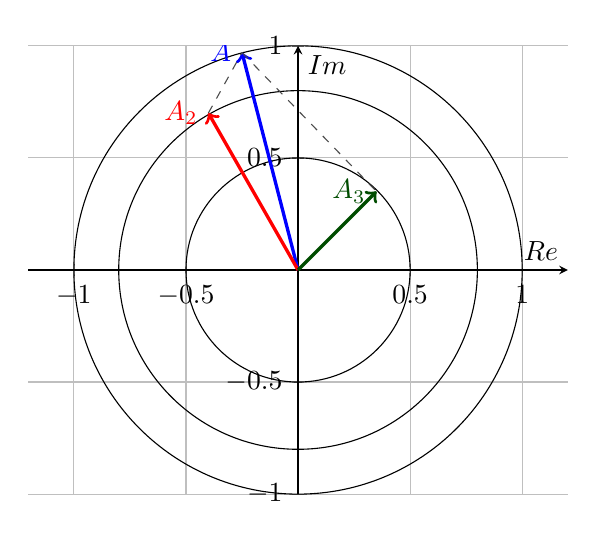
\begin{tikzpicture}
	%\draw[help lines] (0,0) grid (6,4);
	\begin{axis}[axis lines=middle, axis equal, grid=both, xmin=-1, xmax=1, ymin=-1, ymax=1, xlabel = $\operatorname{Re}$, ylabel = $\operatorname{Im}$]
		\draw (axis cs: 0, 0) circle [blue, radius=1];
		\draw (axis cs: 0, 0) circle [red, radius=0.8];
		\draw (axis cs: 0, 0) circle [black!70!green, radius=0.5];
		\addplot[->, blue, very thick] coordinates{(0, 0) (-0.25, 0.97)}  node[sloped, above, blue, left] {$A$};
		\addplot[->, red, very thick] coordinates{(0, 0) (-0.4, 0.7)}  node[sloped, above, red, left] {$A_2$};
		\addplot[->, black!70!green, very thick] coordinates{(0, 0) (0.35, 0.35)}  node[sloped, above, black!70!green, left] {$A_3$};
		\addplot[dashed, black!70] coordinates{(-0.4, 0.7) (-0.25, 0.97)};
		\addplot[dashed, black!70] coordinates{(-0.25, 0.97) (0.35, 0.35)};
	\end{axis}
\end{tikzpicture}